\begin{figure}[hbt!]
    \begin{center}
    \begin{subfigure}[b]{0.6\textwidth}
        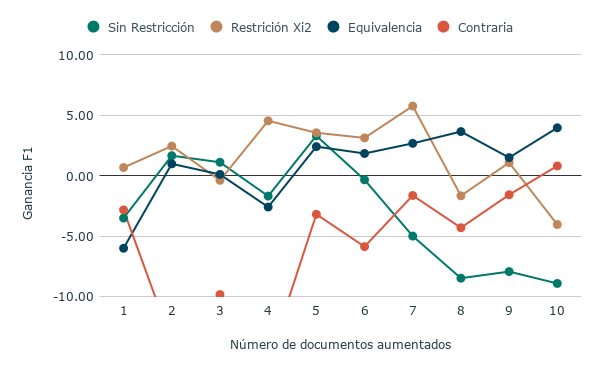
\includegraphics[width=\textwidth]{sections/figures/Bi-LSTM-dep.png}
        \caption{Bi-LSTM}
    \end{subfigure}
    \hfill
    
    \begin{subfigure}[!h]{0.6\textwidth}
        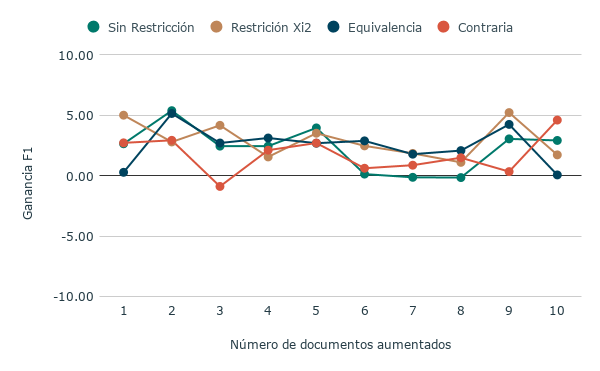
\includegraphics[width=\textwidth]{sections/figures/CNN_dep.png}
        \caption{CNN}
    \end{subfigure}
  
    \begin{subfigure}[b]{0.6\textwidth}
        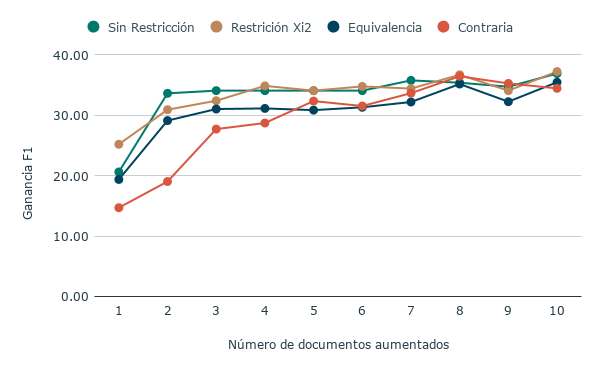
\includegraphics[width=\textwidth]{sections/figures/SVM_dep.png}
        \caption{SVM}
    \end{subfigure}
    \end{center}
   
    \caption{Relación entre el número de documentos aumentados y la ganancia en F1 para el conjunto \textit{Depresión}.}
    \label{fig:aumento_n_depresion}
\end{figure}
